\documentclass[10pt,conference,compsocconf]{IEEEtran}

%\usepackage{times}
%\usepackage{balance}
\usepackage{pdfpages}
\usepackage{url}
\usepackage{graphicx}	% For figure environment
\usepackage{color}
\usepackage{subcaption}
\usepackage{hyperref}
\usepackage{gensymb}

\newcommand{\todo}[1]{{\color{red}{\textbf{TODO: #1}}}}
\newcommand{\conv}[3]{$ \cal{C} $(#1$ \times  $#1, #2, #3)}
\newcommand{\relu}{$ \cal{R}~$}
\newcommand{\maxpool}[2]{$ \cal{M} $(#1$ \times $#1, #2)}
\newcommand{\lrn}{$ \cal{LRN}~$}
\newcommand{\fc}[2]{$ \cal{FC} $(#1, #2)}

\begin{document}
\title{Road Extraction from Aerial Images}
\author{
  Delio Vicini, Matej Hamas, Taivo Pungas\\
  Department of Computer Science, ETH Zurich, Switzerland
}

\maketitle

\begin{abstract}
In this paper, we present a novel method to automatically segment aerial images into road and non-road patches. Our technique classifies small image patches using a deep convolutional neural network. On top of the neural network, we apply a post-processing filter based on a support vector machine classifier. The combination of a convolutional neural network and a post-processing filter yields a $F_1 $ score of over 0.9 on a representative benchmark data set.
\end{abstract}

\section{Introduction}
\label{sec:intro}

Automatically extracting roads from aerial images is a long-standing research topic in computer vision. The solution to this problem has potentially many applications ranging from automation of map making to urban planning and environmental monitoring.

Given an RGB aerial or satellite image, we seek to classify each 16$\times$16-pixel patch as \textit{road} or \textit{non-road}. In the dataset we used, a distance of 1 pixel in the image corresponds to roughly 0.3-0.4 meters.\footnote{Since the used dataset does not come with any scale information, we infer the scale roughly from the size of the observed cars.} This problem is an instance of a binary classification problem. The training data we use to train a binary classifier contains aerial images with corresponding ground truth per-pixel road masks, as shown in Figure \ref{fig:intro_example}.

\par
As aerial image segmentation is a long-standing problem in computer vision with many applications, there is a rich body of previous work in this area \cite{Huang.2002, MnihThesis.2013, Long.2014, Montoya.2015, Saito.2015}. Previous approaches include support vector machines (SVMs) on manually extracted features \cite{Huang.2002}, convolutional neural networks (CNNs) \cite{Long.2014, Saito.2015}, conditional random fields \cite{Montoya.2015} and other probabilistic approaches. Most of the past work has concentrated on per-pixel segmentation. Some papers also look at multi-class semantic classification, e.g. introducing a specific \textit{building} class \cite{Saito.2015}.

Unlike most previous work, we concentrate on per-patch and not on per-pixel prediction. We have developed a novel solution by combining a deep CNN with an SVM-based post-processing algorithm.

We compare our approach to two different baseline algorithms. One of them is a 2-layer CNN with stochastic gradient descent (SGD) optimizer. The second is the same CNN followed by an dictionary-based denoising \cite{Elad.2006} step.

Our main contributions are a patch-based, \mbox{4-layer} CNN architecture for road segmentation and a SVM-based post-processing scheme which further refines predictions produced by the CNN.

\begin{figure}
	\centering
	\begin{subfigure}{.2\textwidth}
		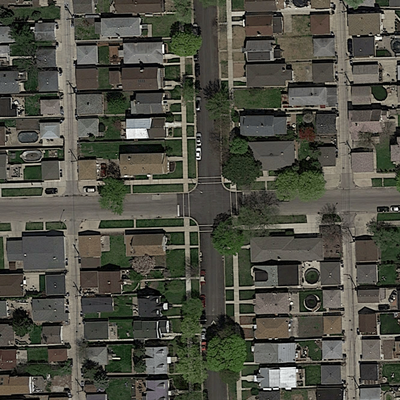
\includegraphics[width=1\textwidth]{figs/img1.png}
	\end{subfigure}
	\begin{subfigure}{.2\textwidth}
		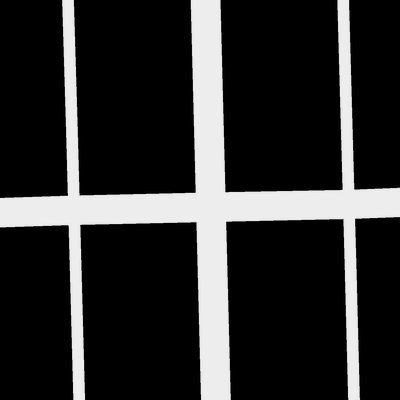
\includegraphics[width=1\textwidth]{figs/groundtruth1.png}
	\end{subfigure}
	\caption{Aerial image of an urban scene and the ground truth road mask.}
	\label{fig:intro_example}
\end{figure}

\section{Models and Methods}
\label{sec:MM}
In this section we describe data augmentation techniques, baseline and final CNN architectures and post-processing techniques applied on the top of the CNN output.

\subsection{Data Augmentation}
\label{subsec:preprocessing}
The lack of training data is a universal problem in machine learning. We extract patches of a particular size from input images. To enlarge the dataset, we generate more training patches by rotating the existing training patches 90 degrees counter-clockwise.

Subsequently, we zero-mean the training dataset by subtracting the mean image from all patches. We do not divide by standard deviation as the images are naturally well distributed.

We then generate the corresponding ground truth patch labels from the given ground truth images. Each ground truth patch is converted to the label 1 if more than one quarter of the pixels in the patch are road pixels; otherwise the patch label is 0. The labels are stored in a 1-hot format, i.e. as tuples \mbox{[0, 1]} or \mbox{[1, 0]}.

Finally, we balance the training dataset to include the same number of positive and negative examples. This is done to prevent the CNN from learning a bias towards one label.

\subsection{Notation - CNN Architecture}
Here, we provide a short overview of CNN layer types that are used in the following sections.
\begin{itemize}
	\item \conv{N}{I}{F} - Convolutional layer with filters of size N$ \times $N, I input channels and F different filters. The number of different filters corresponds to the number of output channels. The default stride is 1 both vertically and horizontally and a clamping boundary condition is used.
	\item \maxpool{N}{S} - Max-pooling layer of size N$ \times $N, stride S.
	\item \lrn - Local response normalization layer across the current batch of training data.
	\item \fc{I}{O} - Fully connected layer from I input channels to O output channels.
\end{itemize}

\subsection{Baseline CNN Architecture}
\label{subsec:baselineCNN}
The baseline CNN operates on patches of size $16 \times 16$. It has two convolutional and two fully connected layers with the following architecture:
\begin{center}
	\conv{5}{3}{32} -- \conv{5}{32}{64} -- \\ 
	\fc{1024}{512} -- ReLU -- \fc{512}{2}.
\end{center}
Each convolutional layer is followed by a rectified linear unit (ReLU) activation layer and a \maxpool{2}{2} max-pooling layer.

The activation functions in the FC layers are identities. We apply \textit{softmax} to two outputs to get the probabilities for both classes. All the weights are initialized normally with standard deviation 0.1. The weights in the FC layers are L2 regularized with a factor $ 5 \times 10^{-4} $. We use a plain vanilla stochastic gradient descent (SGD) optimizer with an exponentially decaying learning rate, starting at 0.01 with a decay rate 0.95. Training samples are processed in batches of 16 samples.

\subsection{Improved CNN Architecture}
\label{subsec:CNN}
We modified the baseline CNN in various ways to improve its performance. We made it deeper, experimented with the widths of layers and filter sizes, tried using dropout or local response normalization instead of L2 regularization of FC weights, tested different optimizers (momentum and Adam \cite{Adam.2014}) and learning rates. We also implemented cross-validation to estimate the training time after which the out-of-sample error converges and subsequently trained the CNN for at least that amount of time.

\begin{figure}
	\centering
	\begin{subfigure}[t]{.15\textwidth}
		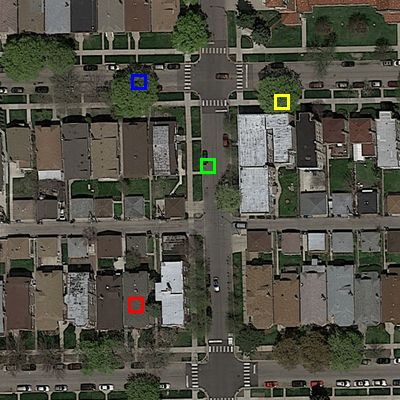
\includegraphics[width=1\textwidth]{figs/context_size/full_img}
		\caption{Input image}
	\end{subfigure}
	\begin{subfigure}[t]{.15\textwidth}
		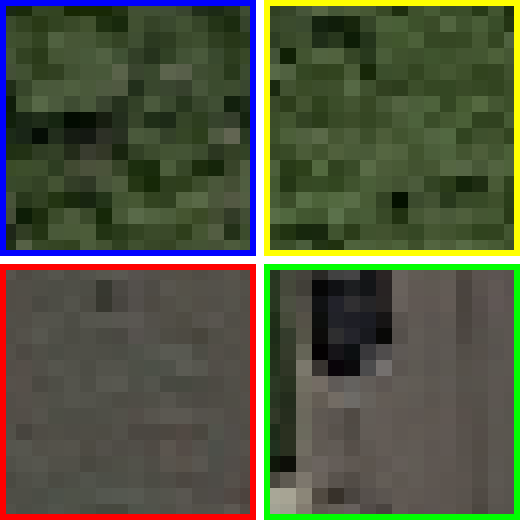
\includegraphics[width=1\textwidth]{figs/context_size/context16}
		\caption{$ 16 \times 16 $ patches}
	\end{subfigure}
	\begin{subfigure}[t]{.15\textwidth}
		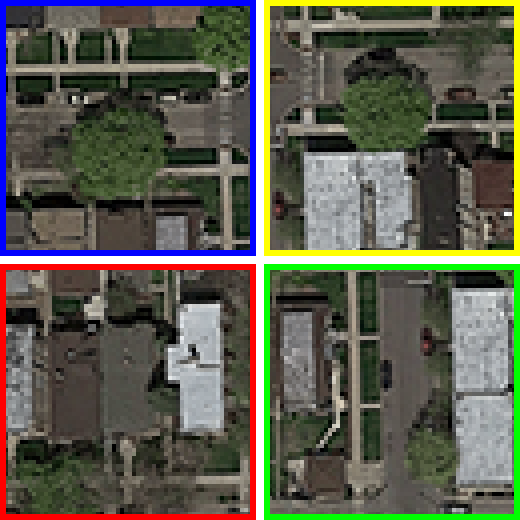
\includegraphics[width=1\textwidth]{figs/context_size/context64_ds}
		\caption{$ 64 \times 64 $ patches (extracted from the downsampled image)}
	\end{subfigure}
	\caption{Aerial image of an urban scene and some example patches. From the $ 16 \times 16 $ context it can be impossible to infer the correct labeling due to the limited perception of the surroundings.}
	\label{fig:context_size}
\end{figure}

Moreover, we increased the context size to $ 64\times64 $, i.e. the network predicts a label for the central $ 16\times16 $ patch using more context. Image boundaries are handled using mirror boundary conditions. Additionally, we downsample training and testing images by a factor of two. This means that the context considered by the neural network effectively doubles. There is no need to use the full high resolution of the input images to reliably predict $ 16 \times 16 $ patches.

\par
Figure \ref{fig:context_size} shows a comparison between the context size of the baseline CNN and the context size of the improved CNN. The yellow and blue patches both show a part of a tree and are extremely similar. However, the blue patch belongs to the part of a tree which covers a road and should be labeled as road, while the yellow patch is not covering the road. The correct labeling can only be inferred by considering a larger context. The red patch could locally easily be mistaken for a road, as its color is very similar to the color of most streets. Even the green patch is hard to predict from the small context, since cars can also occur in non-road areas (e.g. parking lots).

\par
The final architecture of the improved CNN uses four convolutional layers and is structured as follows:
\begin{center}
	\conv{5}{3}{16} -- \conv{3}{16}{32} -- \\ 
	\conv{3}{32}{32} -- \conv{3}{32}{64} -- \\
	\fc{1024}{64} -- ReLU -- \fc{64}{2}.
\end{center}
After every convolutional layer, we apply ReLU, \lrn and \maxpool{2}{2} max-pooling.

The activation function in the first FC layer is the identity function and in the second the sigmoid function. We use neither dropout nor L2 regularization of the FC weights as the local response normalization already sufficiently prevents overfitting. The class probabilities are again obtained using \textit{softmax}. Cross entropy is used as the loss function.

After discovering that exponentially decaying learning rate does not help, we fixed it to the empirically determined value 0.01. 
In the final model, we use the Adam optimizer \cite{Adam.2014} with $ \epsilon = 0.1 $ and the batch size is 32. All the weights are initialized normally using standard deviation 0.1.


\subsection{Post-Processing}
The convolutional neural networks output independent predictions for all $ 16 \times 16 $ patches of the processed image. The spatial arrangement of predictions however contains valuable information, which can be used to further improve the prediction accuracy. For example, it is highly unlikely to observe a road which only covers one patch. If the CNN predicts an isolated patch as belonging to the road label, we can discard this prediction with high certainty. The opposite also holds: a patch labeled as non-road surrounded by patches labeled as road is most likely part of the road as well.

\par 
The simplest post-processing scheme is therefore to simply reject outliers based on the predictions in a 4-neighborhood around the current patch. If all four neighbors of a patch are assigned the label road, we can also assign the label road to the current patch. A simple scheme like this can already significantly improve prediction accuracy, because many prediction errors are isolated outliers. However, more sophisticated algorithms promise even more gain in quality, as the post-processing algorithm should account for more structure than simply the four closest neighbors.

\par 
One more advanced way of reducing the noise in the CNN output is to use dictionary-based denoising \cite{Elad.2006}. We do this by learning a dictionary of 100 atoms, each representing a  $ 5 \times 5 $ square of patch predictions. The dictionary is learned from the patch labels in the training data using the algorithm presented by Mairal et al. \cite{Mairal.2009}. Given the trained dictionary, we can then denoise the predictions for a test image by solving a sparse approximation problem using the orthogonal matching pursuit algorithm for each $ 5 \times 5 $ patch of patch predictions. This is done in a sliding window fashion, similar to the work by Elad et al. \cite{Elad.2006}. We found this to work quite well if the level of noise in the CNN predictions is high, which is the case in the baseline CNN. However, as the quality of the CNN improves, dictionary-based denoising becomes less useful.

\par 
In our pipeline, we filter the CNN output using a binary support vector machine (SVM) classifier. Given a window of $ 7 \times 7 $ patches predicted by the CNN, we predict the label of the central patch using a SVM classifier. We directly use the per-patch probabilities produced by the CNN as features for the SVM classifier. We also tried to automatically extract features using Restricted Boltzmann Machines \cite{smolensky.1986}, but could not achieve an increase in prediction accuracy.
\par
The SVM uses a radial basis function kernel and a soft-margin penalization weight of $ 1 $. We did not perform a systematic search for optimal SVM hyperparameters, as the used parameters seem to work reasonably well.
\par 
We found it beneficial to iteratively apply this denoising technique. This seems to help to propagate confident predictions, as suggested by Mnih and Geoffrey \cite{Mnih.2010}. In practice, we use only two iterations. After two iterations most noise is already removed. Increasing the number of iterations biases the predictions too much and does not lead to a gain in accuracy.

\par
We also tried using graph cut based inference \cite{Boykov.2001}. For this we computed per-pixel labels by accumulating CNN per-patch votes using a sliding window. Graph cut based image segmentation however did not work well, since it relies on strong edges between fore- and background. In our aerial images, this is not the case and the boundary between road and non-road is fairly weak in terms of local edge contrast. Furthermore, the probabilities produced by the CNN are often close to 0 or 1. Graph cut based segmentation is simply not robust enough towards a locally strongly biased data term.

\par 
We also experimented using an additional CNN for post-processing, as suggested by Mnih and Geoffrey \cite{Mnih.2010}. We used a network with two convolutional and two fully connected layers, predicting the central patch from a $ 9 \times 9 $ square of patch predictions from the first CNN. However, we did not get an improvement in accuracy over the simple SVM based post-processing scheme.

\section{Results}
\label{sec:results}
The neural networks were implemented using TensorFlow \cite{tensorflow.2015} and the post processing using scikit-learn \cite{sklearn.2011}. The training set consists of 100 images of a resolution of $ 400 \times 400 $ pixels. For the baseline CNN, we used the code provided in the lecture materials, without any modifications. We trained it for around 30 minutes, which was sufficient to achieve convergence. The training was done on a cluster node with 16 cores (Intel Xeon E5-2697 v2 or Xeon E5-2680 v3 depending on availability on the Euler cluster) and 128GB of memory. We trained our improved CNN model for around 20 hours on the same hardware, which was sufficient to achieve convergence of the loss function. The post-processing SVM trained for around 1.5 hours on a conventional desktop computer (Intel Core2 Quad q9550, 4GB of memory). All neural network code runs exclusively on the CPU, since the used cluster does not provide any GPU nodes. Given the trained models, individual satellite images are processed in a matter of seconds.

\par 
We compare our method to the two different baseline implementations described previously. The first is the CNN described in Section \ref{subsec:baselineCNN}. The second is the same CNN combined with dictionary-based denoising. We measure prediction accuracy as the reported $ F_1 $ score in the public Kaggle leaderboard. Ideally, one would compute an average cross validation error, to also have an estimate of the variance of the measured accuracy. However, since CNNs are very expensive to train we decided to report the Kaggle score only.

\par
The baseline CNN achieves an $ F_1 $ score of only 0.7765. Note that assigning the non-road label to all patches already gives a score of 0.7303. Post-processing the output from the baseline CNN using learned dictionaries improves the $ F_1 $ score to 0.8256. 

\par
Our improved CNN on its own achieves an $ F_1 $ score of 0.8710. Applying our SVM based post-processing procedure on top of these outputs, we reach a score of 0.9020. Note that applying the dictionary-based denoising from the baseline on top of the output of our improved CNN we get an accuracy of only 0.8758.

\begin{figure*}	
	\centering
	\begin{subfigure}[t]{.19\textwidth}
		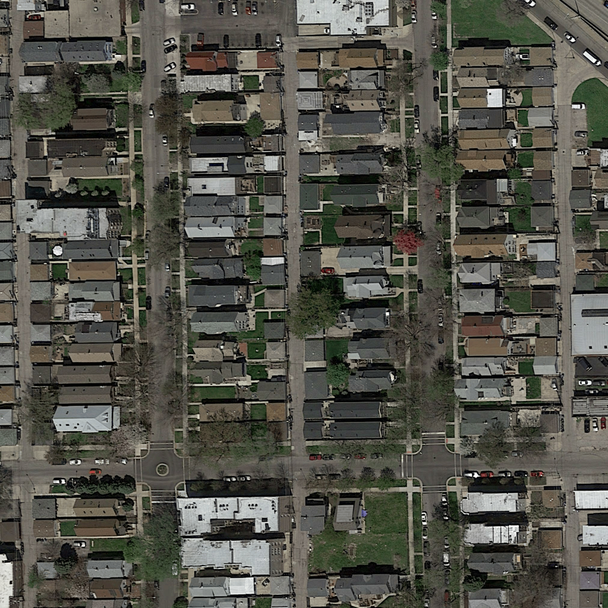
\includegraphics[width=1\textwidth]{figs/results_comparison/input_8}
		\caption{Input image}
	\end{subfigure}
	\begin{subfigure}[t]{.19\textwidth}
		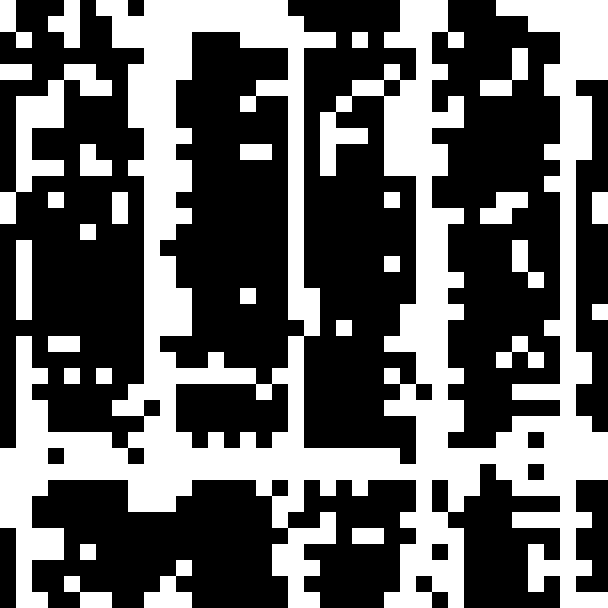
\includegraphics[width=1\textwidth]{figs/results_comparison/cnn_baseline_8}
		\caption{Baseline CNN predictions}
		\label{fig:results_1}
	\end{subfigure}	
	\begin{subfigure}[t]{.19\textwidth}
		
\includegraphics[width=1\textwidth]{figs/results_comparison/post_pro_baseline_8}
		\caption{Denoised baseline CNN predictions}
		\label{fig:results_2}
	\end{subfigure}	
	\begin{subfigure}[t]{.19\textwidth}
		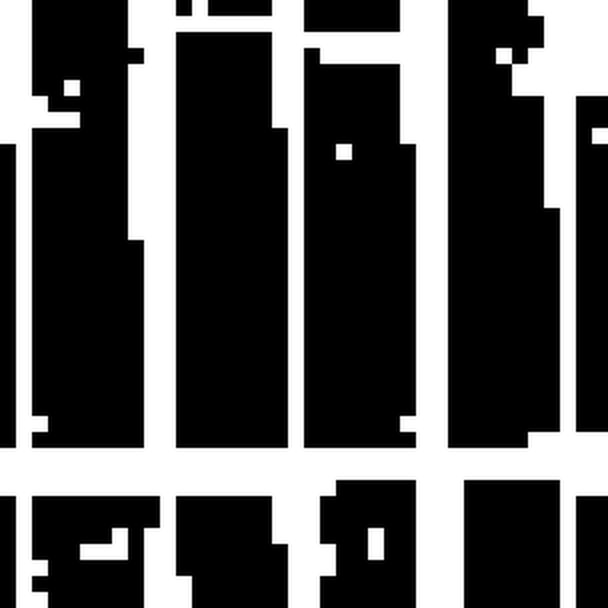
\includegraphics[width=1\textwidth]{figs/results_comparison/cnn_final_8}
		\caption{Improved CNN predictions}
		\label{fig:results_3}
	\end{subfigure}		
	\begin{subfigure}[t]{.19\textwidth}
		
\includegraphics[width=1\textwidth]{figs/results_comparison/post_pro_final_8}
		\caption{Final predictions after SVM-based post-processing}
		\label{fig:results_4}
	\end{subfigure}	
	\caption{Comparison of the results of the two baseline algorithms, the raw output from our improved CNN and our final predictions.}	
	\label{fig:resuls}
\end{figure*}

\section{Discussion}
\label{sec:discussion}
The baseline CNN clearly suffers from the fact that its context size is too small. Given a $ 16 \times 16 $ image patch at the resolutions we worked with, it is oftentimes impossible, even for humans, to correctly decide whether this patch belongs to a road or not. The results of the baseline CNN are therefore very noisy, as seen in Figure \ref{fig:results_1}.

\par 
Adding dictionary-based denoising on top of this baseline CNN improves the predictions. The dictionary-based method manages well with isolated outliers, as shown in Figure \ref{fig:results_2}. However, the prediction quality is inherently limited by the output of the underlying CNN. In contrast to image denoising, the noise produced by the CNN does not have zero-mean. Oftentimes the CNN will mispredict a whole group of patches. The dictionary-based denoising then fails to infer the correct labels. 

\par 
The accuracy gain we achieve using our improved CNN is mostly due to the increased patch size. The larger context reveals much more information about the currently processed image patch. The result shown in Figure \ref{fig:results_3} shows much less noise than the output from the baseline CNN. Despite the improved architecture, there are still many mispredictions. 

\par
Our post-processing algorithm manages to further reduce error. The result in Figure \ref{fig:results_4} shows that almost all noise has been removed. There are still some cases where the post-processing is not very successful. It has a strong bias for roads aligned with the image coordinate axes, since the test set is dominated by these road directions. We experimented with rotating the training images by $ 45\degree $, but did not succeed in improving the prediction accuracy. Our current algorithm often predicts diagonal roads too thin or even removes them partially; an example of this is shown in Figure \ref{fig:post_processing}. This is the most prominent limitation of our current approach. Note, that also the CNN itself does not deal well with diagonal roads.

\begin{figure}
	\centering
	\begin{subfigure}[t]{.15\textwidth}
		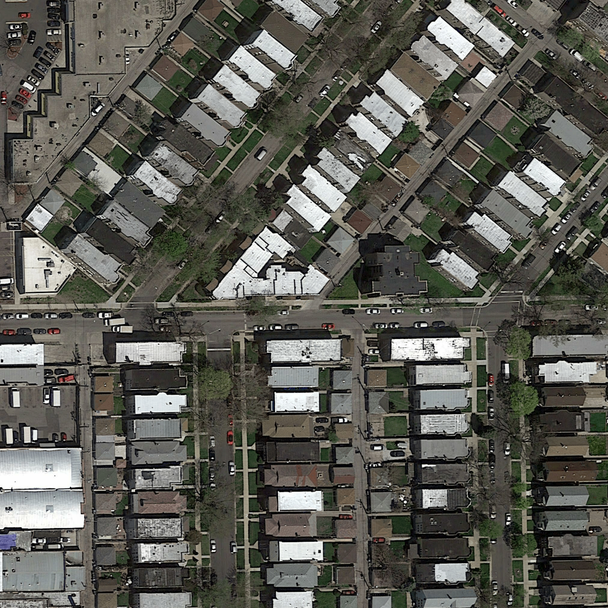
\includegraphics[width=1\textwidth]{figs/post_processing/input}
		\caption{Input image}
	\end{subfigure}
	\begin{subfigure}[t]{.15\textwidth}
		
\includegraphics[width=1\textwidth]{figs/post_processing/cnn}
		\caption{Raw CNN predictions}
	\end{subfigure}
	\begin{subfigure}[t]{.15\textwidth}
		
\includegraphics[width=1\textwidth]{figs/post_processing/postpro}
		\caption{Post-processed predictions}
	\end{subfigure}
	\caption{Results for diagonal roads. Note, that both the CNN and the post-processing algorithm do not deal well with diagonal roads.}
	\label{fig:post_processing}
\end{figure}

\section{Summary}
\label{sec:summary}
In conclusion, we presented an algorithm to automatically extract roads from aerial images. Our algorithm significantly outperforms the two baseline algorithms against which we compared and achieves an $ F_1 $ score of slightly over 0.9. It is particularly strong in images containing mostly roads aligned to the image axes.

\par 
Our algorithm performs worse with images containing mostly diagonal roads. We believe that adding more training images containing diagonal roads should help mitigate this problem. However, the parameters of the neural network and the post-processing then most likely need to be adjusted. 

\par 
Another possible direction of future work would be to jointly predict a set of patches using the CNN instead of independently predicting patches. This could make post-processing less important, since each patch prediction would be influenced by the predictions of the neighboring patches. 

\bibliographystyle{IEEEtran}
\bibliography{references}

\includepdf[pages={1}]{plagiarism_form.pdf}
\end{document}
